\documentclass[12pt,twocolumn]{article}
\usepackage[utf8x]{inputenc}
\usepackage[spanish, es-tabla]{babel}
\usepackage{graphicx}

\usepackage{amsmath}

\title{Proyecto Final}
\author{Juan B. Benavides y Juan P. Vanegas }
\date{\today}

\begin{document}
\maketitle

\section{\label{sec: Intro} Introducción}
La entropía es uno de los conceptos físicos más difíciles de comprender. Para llegar a 
él se puede ver desde el punto de vista termodinámico, o desde un punto de vista más 
cercano a la teoría de la información. A partir de este segundo camino podemos definier la 
entropía como 

\section{Hardware y Software \\ Usado}

\section{Resultados y Análisis}
\begin{figure}
    \centering
    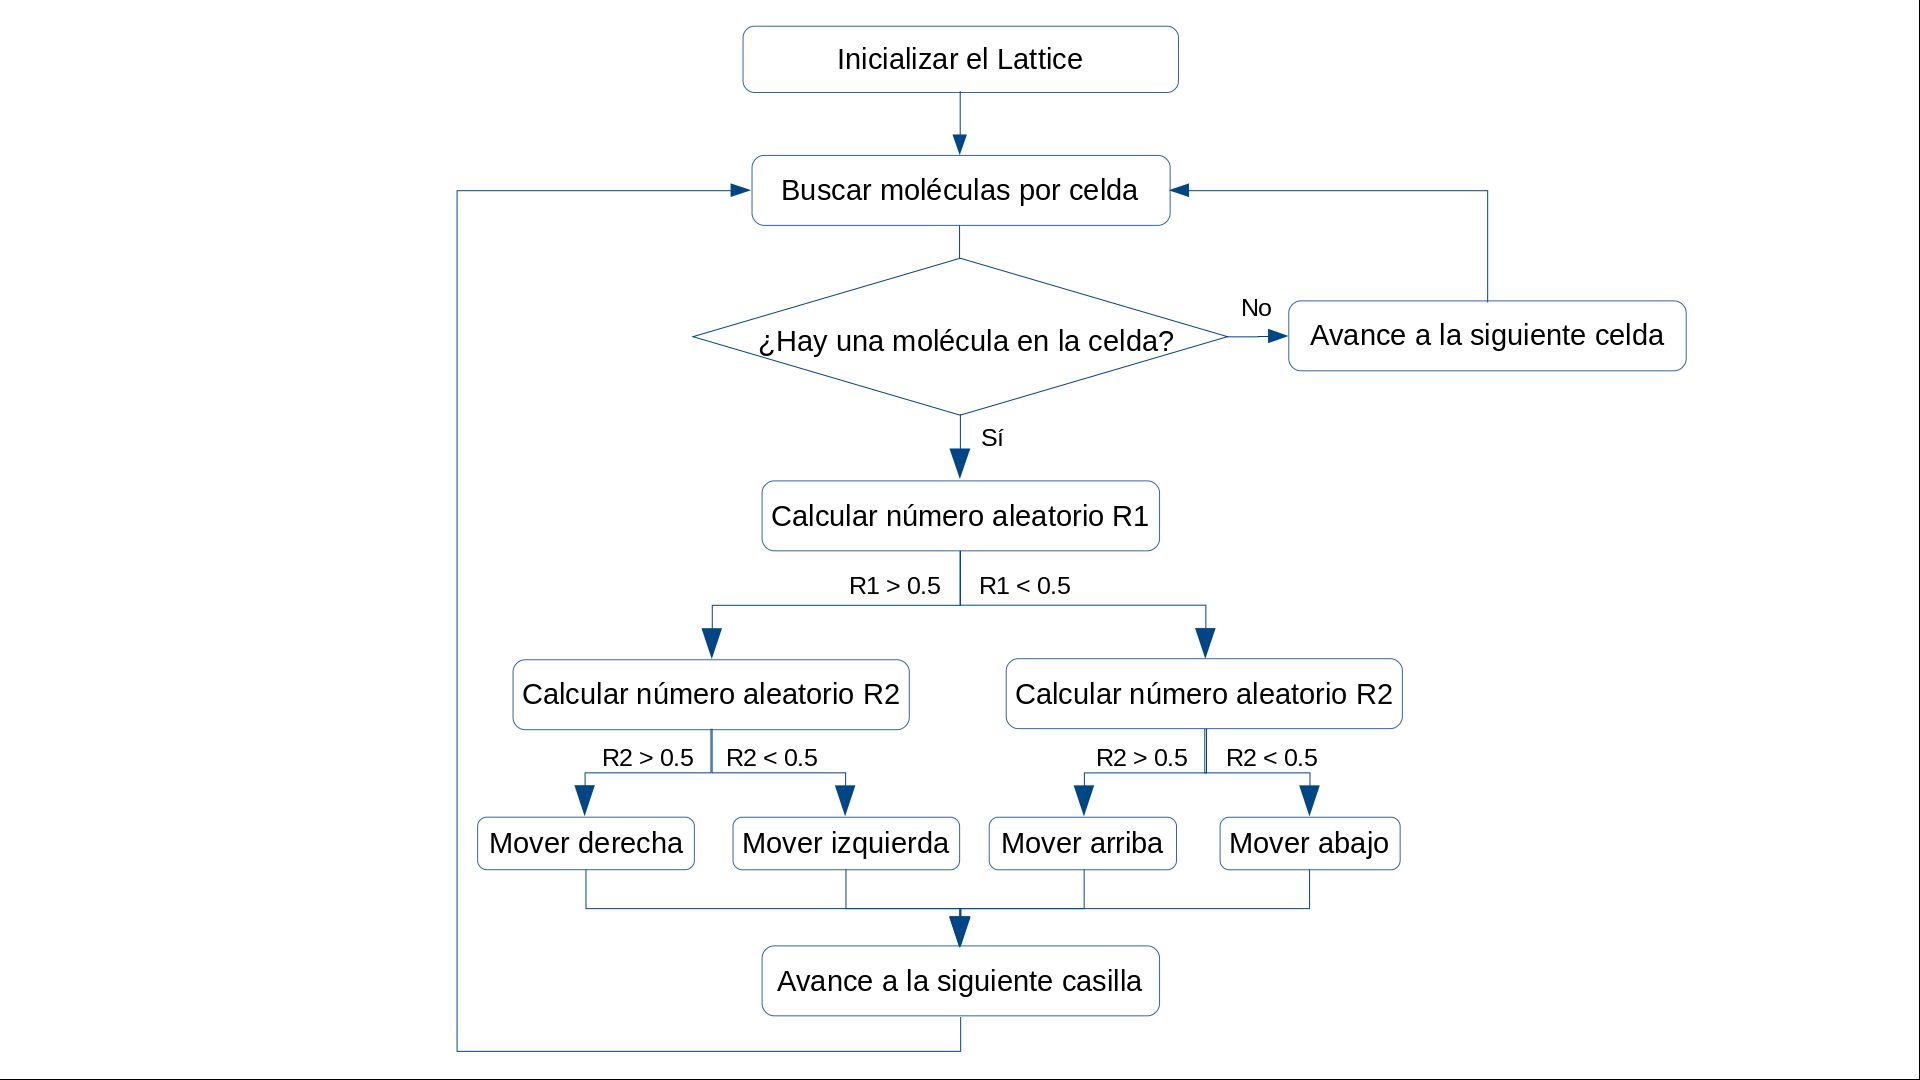
\includegraphics[width=0.3\textwidth]{figs/Algoritmo_OOP.png}
    \caption{Algoritmo 1.}
    \label{fig:algoritmo_OOP}
\end{figure}

\begin{figure}
    \centering
    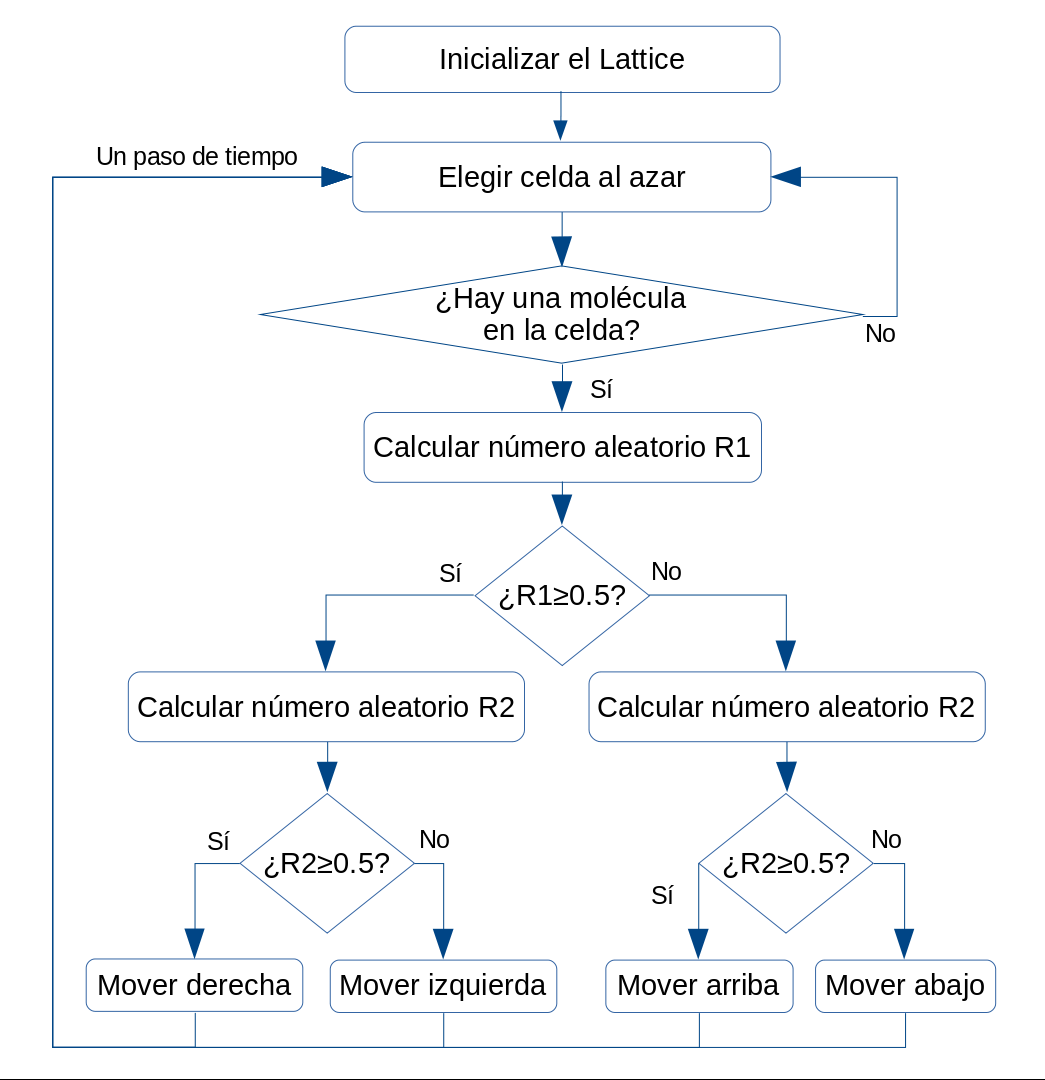
\includegraphics[width=0.3\textwidth]{figs/Algoritmo_Funcional.png}
    \caption{Algoritmo 2.}
    \label{fig:algoritmo_Fun}
\end{figure}

\begin{figure}
    \centering
    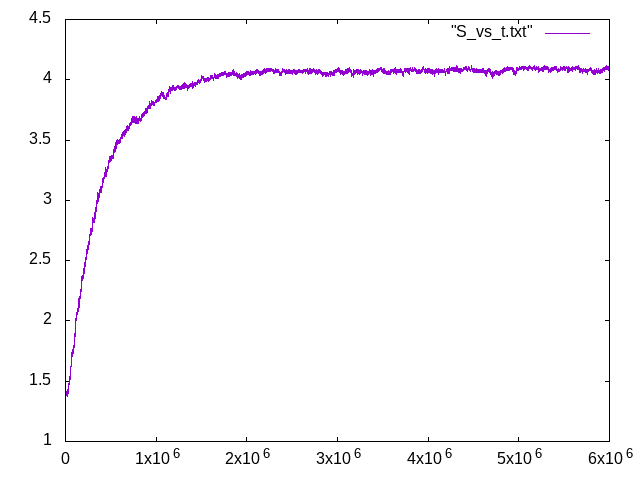
\includegraphics[width=0.3\textwidth]{figs/S_vs_t_OOP_all.png}
    \caption{Entropía en función del tiempo para algoritmo \ref{fig:algoritmo_OOP}.}
    \label{fig:s_vs_t}
\end{figure}


\section{Conclusiones}

\end{document}